\documentclass[11pt, oneside]{article}

\usepackage[english]{babel}
\usepackage{geometry}
\usepackage{graphicx}
\usepackage{tabularx}
\usepackage{amssymb}
\usepackage{amsmath}
\usepackage{booktabs}
\usepackage{xltabular}
\usepackage[hyphens]{url}
\usepackage{hyperref}
\hypersetup{breaklinks=true,hidelinks}
\usepackage[backend=bibtex,style=nature]{biblatex}
\addbibresource{references.bib}

\usepackage{csquotes}
\usepackage{cleveref}
\usepackage{siunitx}
\usepackage{geometry}
\usepackage{multirow}
\geometry{left=4.2cm, right=4.2cm}

\usepackage[dvipsnames]{xcolor}
\definecolor{tumblue}{rgb}{0,0.396078431372549,0.741176470588235}

\usepackage{xspace}
\usepackage{caption}
\usepackage{subcaption}
\usepackage{authblk}
\usepackage{mhchem}


\usepackage{marvosym}

\usepackage{sectsty}

%\usepackage[sort&compress,numbers,super]{natbib}

\sectionfont{\color{tumblue}\selectfont\sffamily}
\subsectionfont{\color{tumblue}\selectfont\sffamily}
\subsubsectionfont{\color{tumblue}\selectfont\sffamily}
\paragraphfont{\selectfont\sffamily}
\subparagraphfont{\color{gray}\selectfont\sffamily}


\renewcommand*{\Authfont}{\sf}
\renewcommand*{\Affilfont}{\sf}


\definecolor{halfgray}{gray}{0.55}
\renewcommand\labelitemi{\color{halfgray}$\bullet$}
%\usepackage{kpfonts}


\clubpenalty = 10000
\widowpenalty = 10000
\displaywidowpenalty = 10000


% if the \fonts folder exists, use fontspec to change fonts
\IfFileExists{./fonts/Heliotrope-Bold.otf}{
    \usepackage{fontspec}
    \setmainfont{Heliotrope}[Extension = .otf, UprightFont = *-Regular, ItalicFont = *-Italic, BoldFont=*-Bold, Path = ./fonts/]
}{
    \usepackage{biolinum}
    \renewcommand{\familydefault}{\sfdefault}
}

\makeatletter
\renewbibmacro*{textcite}{%
  \iffieldequals{namehash}{\cbx@lasthash}
    {\usebibmacro{cite:comp}}
    {\usebibmacro{cite:dump}%
     \ifbool{cbx:parens}
       {\bibclosebracket\global\boolfalse{cbx:parens}}
       {}%
     \iffirstcitekey
       {}
       {\textcitedelim}%
     \usebibmacro{cite:init}%
     \ifnameundef{labelname}
       {\printfield[citetitle]{labeltitle}}
       {\printnames{labelname}}%
     \addspace
     \ifnumequal{\value{citecount}}{1}
       {\usebibmacro{prenote}}
       {}%
     \mkbibsuperscript{\usebibmacro{cite:comp}}%
     \stepcounter{textcitecount}%
     \savefield{namehash}{\cbx@lasthash}}}
\makeatother


\usepackage{lipsum}
\usepackage[labelfont=bf]{caption}

\renewcommand{\Affilfont}{\scriptsize}
 \renewcommand{\Authfont}{\normalsize}

 \usepackage{microtype}


\clubpenalty = 10000
\widowpenalty = 10000
\displaywidowpenalty = 10000

\errorcontextlines=10


\usepackage{tikz}
 \usetikzlibrary{positioning,fit,backgrounds,arrows.meta,calc}
\usepackage{xcolor}


\definecolor{dangercolor}{RGB}{180,30,30} % not used strongly; kept for compatibility
\definecolor{chemcolor}{gray}{0.2}        % not used strongly; kept for compatibility
\definecolor{metacolor}{gray}{0.2}        % not used strongly; kept for compatibility


\usepackage{credits}
\usepackage{orcidlink}
\usepackage{showyourwork}

\title{\textsf{Clever Materials: When Machine Learning Models Fool Themselves}}

\author[1,2, 3, 4, \Letter]{Kevin~Maik~Jablonka~\orcidlink{0000-0003-4894-4660}}



\affil[1]{Laboratory of Organic and Macromolecular Chemistry (IOMC), Friedrich Schiller University Jena, Humboldtstrasse 10, 07743 Jena, Germany}
\affil[2]{Helmholtz Institute for Polymers in Energy Applications Jena (HIPOLE Jena), Lessingstrasse 12-14, 07743 Jena, Germany}
\affil[3]{Center for Energy and Environmental Chemistry Jena (CEEC Jena), Friedrich Schiller University Jena, Philosophenweg 7a, 07743 Jena, Germany}
\affil[4]{Jena Center for Soft Matter (JCSM), Friedrich Schiller University Jena, Philosophenweg 7, 07743 Jena, Germany}



\affil[\Letter]{\texttt{mail@kjablonka.com}}


\begin{document}

\maketitle

\begin{abstract}
Machine learning promises to accelerate materials discovery by uncovering complex structure-property relationships---but what if our models succeed for the wrong reasons? 
Here, I show that across five materials domains—metal-organic frameworks, perovskite solar cells, batteries, and organic electronics—models achieve competitive performance by exploiting bibliographic metadata rather than learning meaningful chemistry. This is the materials science equivalent of the 'Clever Hans' effect: the horse that appeared to calculate but merely read its trainer's cues. Models trained on chemical descriptors predict publication metadata (authors, journals, years) with surprising accuracy, and models using only this predicted metadata often match the performance of conventional structure-property approaches. In predicting the top 10\% most thermally stable metal-organic frameworks, metadata shortcuts prove indistinguishable from descriptor-based models under certain metrics. We have optimized performance without testing why our models work. The path forward requires rigorous evaluation frameworks that falsify competing hypotheses, diverse datasets designed to resist spurious correlations, and honesty about whether we seek chemical understanding or statistical utility. Both have value—but only systematic hypothesis testing, asking not just whether models work but why, elevates pattern matching to science.
\end{abstract}

\section{Introduction}

Machine learning holds both promise and peril for materials discovery. 
The promise lies in its capacity to uncover structure-property relationships too subtle or complex for human recognition.\autocite{hardtrecht2022patterns} 
The peril emerges when models excel by exploiting spurious patterns that collapse under new conditions.\autocite{Lones2024}

This phenomenon---impressive demonstration performance masking fundamental brittleness---represents a classic failure mode in pattern recognition, epitomized by the horse \enquote{Clever Hans}.\autocite{Lapuschkin2019} 
Clever Hans appeared to perform arithmetic calculations, fooling audiences and experts alike, until careful investigation revealed he was simply reading unconscious cues from his questioners. 

Modern machine learning exhibits analogous vulnerabilities. Computer vision models exploit spurious correlations---skin color in medical diagnosis,\autocite{pooch2019trust} background textures in animal classification\autocites{xiao2020noise}---achieving high accuracy through irrelevant shortcuts.\autocite{Brown2023, Howard2021} 
Recent reports from Leash Biosciences suggest similar risks in chemical property prediction: models achieve surprising accuracy at predicting compound provenance, potentially using authorship as a proxy for bioactivity rather than learning meaningful chemistry.\autocite{leash} 

Materials science offers abundant opportunities for such proxy learning (\Cref{fig:clever_hans}). Research groups develop specialized expertise---some focus on solar cell stability optimization, others on MOF synthesis strategies. Laboratory names often appear in framework designations (UiO-66, MIL-101), creating direct author-material associations. 
Fields evolve through paradigm shifts---self-assembled monolayers transforming perovskite cells, post-synthetic modifications revolutionizing MOF properties\autocite{shabih2026autonomous}---embedding temporal signatures that models might exploit rather than learning fundamental chemistry.

\begin{figure}[htb]
	\centering 
	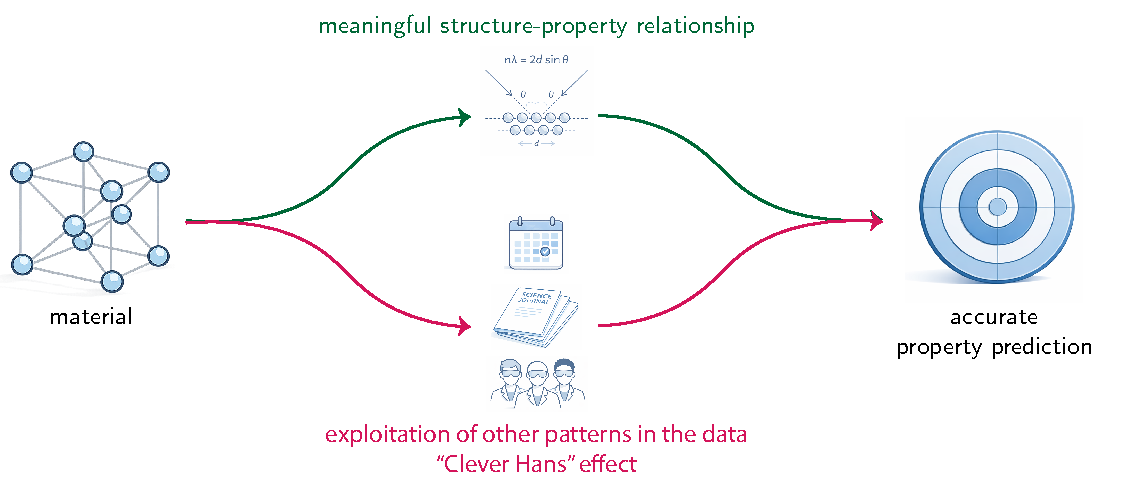
\includegraphics[width=\textwidth]{../static/clever_materials_hans_overview.pdf}
	\caption{\textbf{In machine learning, we often do not test competing hypotheses of how a model might obtain its answers.} Machine learning models in materials science are trained to map material (descriptors) to property predictions. Models have much flexibility in how they learn this map from data. Ideally, they discover robust and meaningful structure-property relationships that also generalize in new settings. This, however, is not guaranteed. Models might also exploit other patterns in the data as a shortcut to a prediction (\enquote{purple}). For instance, it might be easy for the model to spot what researchers produced a given material or in what journal it has been published. Based on those inferences, it might deduce property \enquote{guesses} (as the knowledge of the research group or the publication time can be correlated to the property). The model thus might learn to make good predictions for the wrong reasons. This is known as the \enquote{Clever Hans} effect. The scientific method asks us to test if such alternative patterns can explain good model performance. This is seldom done. In this work, I do it for a few case studies. }	
	\label{fig:clever_hans}
\end{figure}


This work systematically investigates whether commonly used materials datasets are vulnerable to such proxy learning. I augment established property prediction datasets with bibliographic metadata---author names, publication years, journal venues---then test whether models can predict this information from chemical descriptors alone.
The results are sobering: models predict metadata with surprising accuracy, and models using only these predicted \enquote{bibliographic fingerprints} often match the performance of conventional structure-property approaches. 

These findings expose how easily we can be misled about what our models actually learn. More importantly, they point toward concrete strategies for building more robust datasets and developing validation frameworks that actively test competing hypotheses about model performance. 
  


\section{Results}

I systematically assessed Clever Hans vulnerabilities across five materials domains: metal-organic frameworks, perovskite solar cells, battery materials, and organic electronics. Each case study tests whether models can achieve competitive property prediction performance using only bibliographic proxy signals rather than chemical understanding.
Because proxy signal detectability depends critically on prediction task formulation and evaluation metrics, I analyze both regression and classification variants where appropriate, with additional results detailed in the appendix. 

\subsection{MOF Thermal Stability}

Thermal stability represents a critical constraint for MOF applications across gas storage, catalysis, and separation processes.\autocite{Kalmutzki2018} \textcite{Nandy2022} systematically extracted decomposition temperatures from thermogravimetric analyses reported in the literature, creating opportunities to model thermal stability as either a continuous property (regression) or a discrete performance class (classification).\autocite{Nandy2021}

\Cref{fig:mof_thermal_stability} reveals concerning proxy learning capabilities: models predict bibliographic information with high accuracy from structural descriptors alone, then use these predictions to identify thermally elite MOFs (top 10\%) with performance rivaling conventional approaches.

\begin{figure}[htb]
	\centering 
	\includegraphics[width=\textwidth]{figures/mof_thermal_top10_main_panel.pdf}
	\caption{\textbf{For the classification task of membership in the top-10\% of thermally stable MOFs, one can be fooled (by Clever Hans effects).} The model can predict the bibliographic information with high accuracy. \textbf{a} The model predicts the authors of the associated paper with high accuracy, much better than a random baseline. \textbf{b} This also holds for predicting in which journal the entry was published or the year in which the paper was published (\textbf{c}). Using the predicted bibliographic information, a model can also predict with high accuracy if the MOF belongs to the top-10\% thermally stable ones. However, the effect is smaller --- or not even there --- if analyzed under a different metric or for a regression setting. The dummy baseline for classification is a stratified random sampling (using the empirical probabilities from the training dataset) and the mean prediction for the regression case.}
	\label{fig:mof_thermal_stability}	
	\script{analyze-mof-thermal-top10.py}	
\end{figure}




\subsection{MOF Solvent Stability}

Solvent removal stability poses an equally critical challenge for MOF deployment. Many frameworks collapse when synthesis solvents are removed during activation, limiting their practical utility. Using the same text-mined dataset and descriptors,\autocite{Nandy2022} I tested whether proxy signals could predict solvent stability outcomes.

\begin{figure}[htb]
	\centering
	\includegraphics[width=\textwidth]{figures/mof_solvent_main_panel.pdf} 
	\caption{\textbf{Measuring performance using accuracy, \enquote{Clever Hans} models can achieve a surprisingly good performance in predicting solvent removal stability of MOFs.} \textbf{a} MOF descriptors can be used to predict author information better than a random baseline, but not with very high information. \textbf{b} The journal in which a given MOF stability result has been published can also be predicted with non-trivial accuracy. \textbf{c} The publication year can be predicted with a mean average error of two years. \textbf{d} A model trained on predicted bibliographic information can achieve non-trivial accuracy in correctly predicting the solvent stability of MOFs. \Cref{fig:mof_solvent_removal_stability_metric_impact} shows the performance measured with other metrics.}
	\label{fig:mof_solvent_stability}
	\script{analyze-mof-solvent-stability.py}
\end{figure}

\Cref{fig:mof_solvent_stability} demonstrates similar vulnerabilities: descriptors predict bibliographic metadata accurately, and proxy-based models achieve meaningful performance above baseline levels, though not quite matching direct structure-property approaches. This suggests varying degrees of Clever Hans susceptibility across different MOF properties.


\subsection{Perovskite Solar Cell Efficiency}

Perovskite solar cells are another way in which materials scientists aim to have a positive impact on the energy transition.\autocite{CorreaBaena2017}
A metric of central importance here is the power conversion efficiency (PCE). 
It was mined by \textcite{Jacobsson2021} in a manual approach and by \textcite{shabih2026autonomous} in an automated one with large language model-based data extraction.\autocite{SchillingWilhelmi2025} 


\begin{figure}[htb]
	\centering 
	\includegraphics[width=\textwidth]{figures/perovskite_top10_main_panel.pdf}
	\caption{\textbf{\textbf{Clever Hans} models can achieve a high accuracy in predicting if an absorber is within the top-10\% most efficient absorbers.}}
	\label{fig:perovskite_pce_classification}
	\script{analyze-perovskites-top10.py}
\end{figure}

As a case study, I again analyze whether we can predict whether the device belongs to the top 10\% efficient devices. For both the \enquote{Conventional} and \enquote{Clever Hans} models, I derive descriptors for the composition of the absorber. 



\subsection{Battery Capacity}

For sustainability, energy does not only need to be converted. For this, batteries are important. \textcite{Huang2020} text-mined battery materials alongside performance metrics. 

\begin{figure}[htb]
	\centering 
	\includegraphics[width=\textwidth]{figures/battery_main_panel.pdf}
	\caption{Battery capacity}
	\label{fig:battery_capacity}
	\script{analyze-batteries-top10.py}
\end{figure}

\Cref{fig:battery_capacity} shows that while the model can predict bibliographic information better than the random baseline based on the composition features, it still does so with relatively low performance.
The prediction of the publication year shows higher performance.


\subsection{TADF Emitter Properties}

Thermally activated delayed fluorescence (TADF) is one mechanism to improve the efficiency of organic light-emitting diodes (OLED)s.\autocite{Liu2018} The maximum emission wavelength is one important performance metric that is optimized for these materials. \textcite{Huang2024} text-mined using ChemDataExtractor.\autocite{Swain2016, Mavrai2021}

As a feature set for the \enquote{Conventional} and \enquote{Clever Hans} models, I use a broad set of molecular descriptors and fingerprints. Both \enquote{Conventional} and \enquote{Clever Hans} models aim to predict the maximum emission wavelength. 

\begin{figure}
	\centering
	\includegraphics[width=\textwidth]{figures/tadf_main_panel.pdf}
	\caption{\textbf{\enquote{Clever Hans} models perform worse than \enquote{conventional} models but better than simple baselines in predicting the maximum emission wavelengths of TADF molecules.} \textbf{a} Using composition descriptors, the model can predict the the authors of the paper describing a material with an accuracy of \protect\input{output/tadf_best_meta_accuracy.txt}  among the 1000 most profilic authors. \textbf{b} The model achieves an even higher performance in predicting in which of the ten most common journals a given entry has been published. \textbf{c} The publication year, too, can be predicted with a high performance just based on composition descriptors. \textbf{d} Using predicted bibliometric information, the authors achieve a mean absolute error between the \enquote{Conventional} and naïve baseline models.}
	\label{fig:tadf_main}
	\script{analyze-tadf.py}
\end{figure}


\subsection{Overall effects}

In the analysis, I find that not in all cases, shortcut learning via bibliometric information can perform competitively with \enquote{conventional} models. 
But it still, shortcut learning via predicted bibliometric information often performed surprisingly well. 
Whether one could detect it or not depended on the choice of baseline and metric. 


\section{Discussion}

Machine learning has transformed materials discovery,\autocite{Moosavi2020, Saal2020, Gubernatis2018} but the findings here highlight a critical gap: we often fail to rigorously test alternative hypotheses for why our models perform well. 
The scientific method demands that we actively seek to falsify our hypotheses,\autocite{Platt1964, popper2005logic, Chamberlin1965} yet in machine learning, we tend to focus on optimizing performance rather than exploring competing explanations.

The Clever Hans effect represents just one class of alternative hypotheses we should systematically explore. 
When we claim that models \enquote{learn meaningful chemistry,} we must test whether simpler explanations --- such as shortcuts via author identity or publication date --- could account for the observed performance.\autocite{Chuang2018} 
This requires a shift from asking \enquote{does this model work?} to \enquote{why does this model work, and what are all the ways it could be wrong?}

The space of potential confounders is vast and often non-obvious. Beyond the shortcuts via meta-information investigated in this work, models might exploit dataset construction artifacts, measurement biases, or many other spurious effects.\autocite{Zhou2025, Jones2024} 
Systematically exploring these alternatives is computationally intensive but crucial for scientific rigor.

LLM-based agents might offer a promising approach to automate this exploration.\autocite{Ramos2025, alampara2025general} 
These systems could generate and test competing hypotheses in parallel, exploring the space of potential explanations more thoroughly than human researchers typically manage. 
Such agents could serve as \enquote{devil's advocates,} systematically challenging our assumptions about why models succeed.

\subsection{Toward Robust Materials Data Infrastructure}

Another angle is to reconsider how we generate, curate, and share materials data. 
The field needs coordinated infrastructure that prioritizes diversity and robustness over convenience. \autocite{Krishnan2025}
Convenience and short-term reward are often too easy and compelling to optimize for due to collective action problems trapping an ecosystem in a suboptimal state, where every actor knows that changes would be needed, but no one wants to make the first move.\autocite{Nielsen2020-rr} 

Most automated screening approaches optimize specific objectives using limited building blocks, which creates exactly the kind of proxy signals that models learn to exploit. And also human researchers are biased in how they explore chemical space.\autocite{Jia2019}
Organizations that can generate diverse data at scale---potentially focused on the lowest cost per reproducible data point rather than pushing particular research agendas---might help to address this problem. 

But it is important to keep in mind that in some circumstances, we will never be able to acquire \enquote{enough} data. Thus, we also need renewed focus on how we evaluate models.\autocite{goldman2024statistical} 
Instead of asking whether models work, we should ask why they work and systematically explore alternative explanations. 
This means actively trying to disprove our own --- but also others' --- claims about model performance.
To enable others to do so, access to data and code is obviously a prerequisite. But one could also envision that some of these tests might require new experiments --- which could be facilitated using infrastructure as a service or incentivized using \enquote{bug bounties} for research papers, models, or datasets. We need to accept that receiving feedback --- even if it is pointing out a mistake in our own work --- is a gift.

\section{Conclusions}

Model evaluation has always been challenging in materials science.\autocite{Alampara2025} 
We have developed increasingly sophisticated techniques to address this: time-based splitting,\autocite{sheridan2013time, Landrum2023} scaffold splits, leave-one-cluster-out cross-validation,\autocite{Durdy2022, Meredig2018} cluster-based splits,\autocite{guo2024scaffold} and property-based splits.\autocite{Jablonka2023, kunchapu2025polymetrix} 
In some domains, even challenges have been organized.\autocite{Moult2005, Tetko2024, Llinas2019}
Each technique revealed new ways that models could fail to generalize, forcing us to be more rigorous in our evaluation practices.

This work highlights yet another layer of complexity. 
Models can achieve impressive performance not by learning meaningful chemistry, but by exploiting subtle biases in how our datasets are constructed. Across five different materials domains, I find that proxy signals---such as shortcut learning via publication meta-information---can provide substantial predictive power.

The simplest explanation for good model performance might often be shortcut learning, not meaningful understanding of chemistry. 
This is an uncomfortable truth, but the space of potential confounders extends far beyond what current evaluation techniques can catch.

Like the original Clever Hans, our models may be performing impressive feats---but for all the wrong reasons. 
They excel not because they understand chemistry, but because they have learned to read the subtle clues inadvertently embedded in our data. 
Thus, we should not only ask whether our models can achieve good performance, but also whether we can trust what that performance actually means.

This is not necessarily a condemnation of all shortcut learning. 
Models that exploit proxy signals can still provide statistically reliable predictions and practical value---as long as the underlying patterns remain stable and as long as we only care about the average performance. 
The critical issue is transparency about what we are doing and why.

If our goal is scientific understanding and robust generalization to genuinely new materials, we must systematically explore alternative explanations and build models that resist spurious correlations. 
If our goal is simply a predictive tool that works well on average, we can accept some brittleness---but we should communicate openly that the model may fail in unpredictable ways when the hidden assumptions break down.

In the end, the Clever Hans problem forces us to confront a choice about scientific machine learning: Do we want tools that advance chemical understanding, or are we content with sophisticated pattern matchers that reflect various biases and artifacts? 
Both approaches can have merit, but honesty about which path we are taking will help to unlock real acceleration using machine learning. 

\section{Methods}

\subsection{Clever Hans Analysis Framework}

I implemented a systematic framework to quantify Clever Hans effects in materials property prediction. For each dataset, I trained three types of models: (1) conventional models that predict material properties directly from chemical descriptors, (2) indirect models that first predict meta-information (author identity, journal, publication year) from the same descriptors and then use these predictions to estimate material properties, and (3) dummy baselines using stratified sampling for classification or mean prediction for regression.

The indirect prediction approach tests whether meta-information contains sufficient signal to achieve competitive prediction performance. If models can predict material properties as accurately using only proxy information as using chemical descriptors, this indicates potential Clever Hans effects in the dataset.

\subsection{Model Architecture and Training}

All models used gradient boosting, implemented with \texttt{LightGBM}\autocite{lightgbm} with default hyperparameters. 

\subsection{Cross-Validation Protocol}
I used 10-fold cross-validation with random shuffling unless otherwise mentioned. Individual dots in swarm plots indicate the performance on the individual folds. 
For each of the 10 cross-validation folds, I maintain strict separation between training and testing phases: In the training phase, three models are trained simultaneously on the same training data: (1) the conventional model learns to map chemical descriptors directly to target properties, (2) the meta-prediction model learns to predict bibliographic information (authors, journals, publication years) from chemical descriptors, and (3) the proxy model learns to map predicted bibliographic information to target properties.
In the testing phase, the conventional model predicts properties from descriptors on the held-out fold. 
The meta-prediction model generates bibliographic predictions for the test materials, and the proxy model uses the predicted bibliographic data (not ground-truth metadata) to predict properties.
This protocol ensures that proxy models cannot access ground-truth bibliographic information during testing, only their own uncertain predictions. The comparison thus reflects realistic deployment scenarios where future materials would lack known authorship or publication context.

\subsection{Datasets and Feature Engineering}

\subsubsection{Battery Dataset}
I obtained the battery dataset from \textcite{Huang2020}

The battery dataset contained \input{output/battery_dataset_size.txt} entries with \input{output/battery_n_features.txt} chemical descriptors.

\subsubsection{Perovskite Dataset} 
I obtained the perovskite dataset from \textcite{shabih2026autonomous}, which is based on \textcite{Jacobsson2021}.

The perovskite dataset contained \input{output/perovskite_dataset_size.txt} entries with \input{output/perovskite_n_features.txt} descriptors.

\subsubsection{MOF Datasets}
I obtained the MOF datasets from \textcite{Nandy2022}. The dataset already contains precomputed features such as revised autocorrelation functions.\autocite{Moosavi2020} 

The MOF thermal stability dataset contained \input{output/mof_thermal_dataset_size.txt} entries with \input{output/mof_thermal_n_features.txt} structural and chemical descriptors. 
The MOF solvent stability dataset contained \input{output/mof_solvent_dataset_size.txt} entries with \input{output/mof_solvent_n_features.txt} descriptors.
I used the MOF descriptors provided by \textcite{Nandy2022}. 

\subsubsection{TADF Dataset}
I obtained the TADF dataset from \textcite{Huang2024}. 
The TADF dataset contained \input{output/tadf_best_dataset_size.txt} entries with \input{output/tadf_n_features.txt} molecular descriptors. As inputs for the models, I used compositional descriptors.

\subsection{Chemical Descriptor Generation}

For datasets containing molecular or compositional information, I generated comprehensive chemical descriptors to serve as baseline features for property prediction. 

\subsubsection{Molecular Descriptors from SMILES}
For datasets with SMILES (Simplified Molecular-Input Line-Entry System) strings,\autocite{Weininger1988} I computed molecular descriptors using RDKit \autocite{rdkit}. The molecular feature set included:

\begin{itemize}
    \item \textbf{2D descriptors}: All available RDKit molecular descriptors ($\sim$200 features), including molecular weight, LogP, topological polar surface area, number of aromatic rings, hydrogen bond donors/acceptors, and rotatable bonds.
    \item \textbf{Fingerprints}: 2048-bit circular fingerprints with radius 2, capturing local chemical environments and structural motifs.
\end{itemize}

Molecules were parsed from SMILES strings, and invalid or unparseable structures were excluded. 
\subsubsection{Composition Descriptors}
For datasets with chemical formulas (battery materials, perovskites), I computed composition-based descriptors using matminer \autocite{matminer}. The composition feature set included:

\begin{itemize}
    \item \textbf{Element properties}: Elemental statistics (mean, standard deviation, range) for atomic properties, including atomic radius, electronegativity, ionization energy, and electron affinity using the Magpie preset \autocite{ward2016general}.
    \item \textbf{Stoichiometric features}: Composition statistics including element fractions, number of components, and chemical complexity metrics.
    \item \textbf{Meredig descriptors}: Extended element property statistics including orbital contributions and chemical bonding characteristics \autocite{meredig2014combinatorial}.
\end{itemize}

Chemical formulas were parsed using pymatgen \autocite{pymatgen}, and compositions that could not be parsed were excluded from analysis. 

\subsubsection{Feature Processing}
Generated descriptors were processed to handle missing values and ensure numerical stability for gradient boosting models. Features with excessive missing values ($>$50\%) were excluded, and remaining missing values were imputed with feature medians. For XGBoost and LightGBM models, additional preprocessing included clipping extreme values to prevent numerical overflow and replacing infinite values with conservative bounds.

\subsection{Meta-Information Extraction}

I enriched the datasets with publication meta-information using the Crossref API to retrieve bibliographic data, including author names, journal titles, and publication years. I created binary features indicating the presence of the top-$N$ most frequent authors and journals in each dataset, where $N$ was varied across 10, 50, 100, and 500 (or maximum available).

\subsection{Data Processing}

All datasets were preprocessed to remove entries with missing target values or author information.




\subsection*{Data Availability}

The datasets used in this study are available on Zenodo: [DOI placeholder].

\subsection*{Code Availability}

All analysis code is available on GitHub: [URL placeholder].

\section*{Acknowledgement}
This work was supported by the Carl Zeiss Stiftung. The author is a member of the NFDI consortium FAIRmat - Deutsche Forschungsgemeinschaft (DFG) - Project 460197019.

\section*{Declaration of Generative AI and AI-assisted Technologies in the Research and Writing Process}
I used Anthropic's Claude models as \enquote{copilot} in code development. I also used those models to improve language and readability. After using this service, I reviewed and edited the content as needed and take full responsibility for the content of the publication.

\printbibliography

\pagebreak


\appendix

\section{Detailed Results}
In this section, I show performance for metadata and property prediction in more detail. 


\subsection{MOF Solvent Removal Stability}

\begin{figure}
	\includegraphics[width=\textwidth]{figures/mof_solvent_performance_comparison.pdf}
	\label{fig:mof_solvent_removal_stability_metric_impact}
	\script{analyze-mof-solvent-stability.py}
\end{figure}

\clearpage

\subsection{MOF Thermal Stability}

\begin{figure}
	\includegraphics[width=\textwidth]{figures/mof_thermal_top10_performance_comparison.pdf}
	\caption{\textbf{MOF stability prediction performance under different metrics.}}
	\label{fig:mof_thermal_stability_metric_impact}	
	\script{analyze-mof-thermal-top10.py}	
\end{figure}


\clearpage

\subsection{Perovskite Regression}
\Cref{fig:perovskite_main_regression} shows the \enquote{Clever Hans} behavior in the regression case. 
\Cref{fig:perovskite_parameter_sweep_regression} shows the predictive performance as a function of the number of bibliometric features. 

\begin{figure}
	\centering
	\includegraphics[width=\textwidth]{figures/perovskite_main_panel.pdf}
	\caption{\textbf{Performance in predicting bibliometric information and in predicting photoconversion efficiencies.}}
	\label{fig:perovskite_main_regression}
	\script{analyze-perovskites.py}
\end{figure}

\begin{figure}
	\centering
	\includegraphics[width=\textwidth]{figures/perovskite_parameter_sweep.pdf}
	\caption{\textbf{Impact of the number of bibliometric features on the performance of \enquote{Clever Hans} models in predicting PCE.}}
	\label{fig:perovskite_parameter_sweep_regression}
	\script{analyze-perovskites.py}
\end{figure}



\end{document}
